\documentclass[conference]{IEEEtran}

\usepackage{amsmath}
\usepackage{booktabs}
\usepackage{graphicx}
\usepackage{multirow}
\usepackage{xcolor}
\usepackage{url}

\graphicspath{{../hls_ml/figures/}}

\title{Reliability-Aware Multi-Objective HLS QoR Prediction Under Kernel-Level Distribution Shift}

\author{
\IEEEauthorblockN{AUTHOR NAME(S)}
\IEEEauthorblockA{
Department or Laboratory\\
University or Organization\\
City, Country\\
email@example.com}
}

\begin{document}
\maketitle

\begin{abstract}
Machine-learning models can accelerate high-level synthesis (HLS) design-space exploration by predicting quality-of-result (QoR) metrics before expensive synthesis. However, random row-level evaluation can be optimistic when multiple pragma configurations of the same kernel are distributed across training and test sets. This paper presents a reliability-oriented evaluation of multi-objective HLS QoR prediction under kernel-level distribution shift. Using the released ForgeHLS data and its embedded synthesis-derived measurements, we audit 184,717 records, construct 42 deterministic source/configuration features, and predict worst-case latency, LUT, DSP, FF, and BRAM\_18K usage. We compare random row splits with group-disjoint splits defined by source--algorithm kernel groups, repeat the disjoint experiment over five seeds, and evaluate tree disagreement and deep-ensemble uncertainty. We additionally measure interval coverage, calibration error, and risk--coverage behavior. The audited release contains 491 logical kernel groups, and every grouped split has zero train--test group overlap. Under the disjoint protocol, latency remains the most predictable target, while resource-target generalization is weak and target-dependent. Tree disagreement is strongly associated with absolute error, with Spearman correlations of 0.887--0.976 across the five targets in the verified run. At the same time, calibration is not uniformly reliable, particularly for heavy-tailed latency and zero-heavy resources. These results show that HLS QoR predictors should be assessed not only by point accuracy but also by distribution shift, uncertainty ranking, calibration, and selective prediction.
\end{abstract}

\begin{IEEEkeywords}
high-level synthesis, quality of result, distribution shift, uncertainty quantification, calibration, selective prediction, trustworthy machine learning
\end{IEEEkeywords}

\section{Introduction}
High-level synthesis translates algorithmic C/C++ descriptions into hardware implementations. A single source program can generate many implementations through pragma and configuration choices, creating a large design space in which synthesis is expensive. Learned QoR predictors are therefore attractive as surrogate models for design-space exploration (DSE). The central practical question, however, is not only whether a model fits previously observed kernel families. It is whether its prediction can be trusted when the next kernel has not appeared in the training data.

Many benchmark evaluations use random row splits. Such a split is convenient, but it can place different configurations of the same logical kernel in both partitions. The test set then measures interpolation among related configurations rather than generalization to an unseen kernel. This distinction is related to broader work on evaluation under distribution shift and group shifts \cite{koh2021wilds,sagawa2020distributionally,chen2021mandoline}. It is especially important for HLS because pragma variants of one program can be numerous and highly correlated.

This paper studies that reliability problem using the ForgeHLS dataset \cite{peng2025forgehls}. We treat the source--algorithm pair as a logical kernel group and compare an intentionally optimistic random row split with kernel-disjoint evaluation. We report five-seed repeated results, raw and log-scale errors, uncertainty--error association, interval calibration, and selective prediction. We also include validation-only tuning as a secondary analysis rather than presenting it as a universally superior predictor.

The contributions are:
\begin{itemize}
    \item an auditable, leakage-controlled protocol for HLS QoR prediction under kernel-level distribution shift;
    \item a multi-objective evaluation covering latency and four implementation-resource targets on real synthesis-derived records;
    \item a reliability analysis combining tree disagreement, deep-ensemble variance, calibration, and risk--coverage evaluation; and
    \item an evidence-based characterization of where tuning helps, where it does not, and why target-wise claims are safer than universal accuracy claims.
\end{itemize}

\section{Related Work}
\subsection{HLS QoR prediction}
ForgeHLS provides a large open dataset of HLS source/configuration records and synthesis-derived QoR measurements \cite{peng2025forgehls}. Automated HLS exploration systems such as AutoDSE demonstrate the practical value of reducing manual pragma tuning \cite{sohrabizadeh2022autodse}. Classical regressors, tree ensembles, and neural predictors have been used as surrogates for HLS exploration. This paper does not claim that the use of a standard regressor is itself novel. Instead, the focus is the validity and reliability of evaluation when kernel identity is a source of dependence.

\subsection{Uncertainty and selective prediction}
Ensemble disagreement and predictive variance are commonly used as practical uncertainty surrogates. Random forests provide a natural disagreement signal across trees \cite{breiman2001random}, while deep ensembles provide a complementary predictive-variance estimate \cite{lakshminarayanan2017simple}. Predictive intervals can be evaluated through coverage, width, and calibration error \cite{guo2017calibration,kuleshov2018accurate}. Conformal methods provide a distribution-free framework under appropriate exchangeability assumptions \cite{vovk2005algorithmic,angelopoulos2023conformal,romano2019conformalized}, while selective classification formalizes the trade-off between coverage and risk \cite{geifman2017selective}. Under dataset shift, uncertainty quality can change substantially \cite{ovadia2019can}. Our study uses these ideas as evaluation tools and explicitly reports when calibration is target-dependent.

\section{Dataset and Feature Construction}
\subsection{Observed data}
The verified downloaded ForgeHLS release contains 184,717 records, 11 unique sources, 471 algorithm names, 491 source--algorithm groups, 1,242 design identifiers, and 3,803 Pareto records. The core audit found no missing required fields. Each record contains source/configuration information and five synthesis-derived targets:
\[
\mathbf{y}=[\text{Worst-caseLatency},\text{LUT},\text{DSP},\text{FF},\text{BRAM\_18K}].
\]
The experiments use the real JSON release and regenerate the feature and split artifacts in the Colab workflow; no synthetic records or imputed target values are introduced.

\subsection{Features}
The feature extractor produces 42 deterministic features. Set A contains basic timing and source-size quantities. Set B adds pragma-aware counts and indicators, including pipeline, unroll, partition, reshape, dataflow, inline, resource, binding, and storage-related features. Set C adds source-structure quantities such as functions, loops, branches, arrays, operators, memory accesses, and nesting depth. Source names, algorithm names, design identifiers, and target-derived strategy labels are not used as model inputs.

\section{Evaluation Protocol}
\subsection{Grouping and splits}
We define a logical kernel group as
\[
g=(\text{source\_name},\text{algo\_name}).
\]
E1 is an 80/20 random row split with seed 42. E2 is an 80/20 group-disjoint split using the same grouping rule. E3 repeats group-disjoint evaluation with seeds 42--46. Each E3 split contains 392 training groups and 99 test groups, with zero group overlap. E1 is retained as a diagnostic of optimism, not as the primary estimate of deployment performance.

\subsection{Models and metrics}
The baseline comparison includes Ridge regression, Random Forest \cite{breiman2001random}, Gradient Boosting \cite{friedman2001greedy}, and an MLP. Separate regressors are fit for each target. We report $R^2$, MAE, normalized MAE, median absolute error, and log-MAE. Log-MAE is emphasized because latency is heavy-tailed and DSP/BRAM are zero-heavy. Validation-only tuning compares compact Random Forest and Gradient Boosting configurations. The tuned results are reported as secondary evidence and are not selected by inspecting the E3 test results.

\subsection{Uncertainty, calibration, and selective prediction}
For tree disagreement, uncertainty is the standard deviation of tree-level predictions. For the deep ensemble, uncertainty is the variance of five independently initialized predictors. We evaluate Spearman correlation between uncertainty and absolute error, compare the lowest and highest uncertainty quintiles, and compute 50--95\% interval coverage. We also generate risk--coverage curves by accepting the lowest-uncertainty predictions first.

\section{Results}
\subsection{Distribution shift}
Table~\ref{tab:e1e2} summarizes the representative E1 and E2 results for Random Forest and Gradient Boosting. Random row splits are substantially more favorable for resources than kernel-disjoint evaluation. For example, Random Forest LUT $R^2$ decreases from 0.273 to -0.043, DSP from 0.226 to -0.372, and BRAM from 0.852 to -0.024. Gradient Boosting is the strongest fixed baseline for E2 latency with $R^2=0.782$, but its resource $R^2$ values remain close to zero or negative.

\begin{table*}[t]
\centering
\caption{Representative E1 random-row and E2 kernel-disjoint results from the verified real-data run. Values are $R^2$; E2 LogMAE is shown in parentheses.}
\label{tab:e1e2}
\begin{tabular}{llrrrr}
\toprule
Model & Metric & Latency & LUT & DSP & FF & BRAM\\
\midrule
Random Forest & E1 $R^2$ & 0.965 & 0.273 & 0.226 & 0.160 & 0.852\\
Random Forest & E2 $R^2$ & 0.731 & -0.043 & -0.372 & 0.012 & -0.024\\
Random Forest & E2 LogMAE & 1.774 & 0.845 & 0.853 & 1.138 & 0.464\\
Gradient Boosting & E1 $R^2$ & 0.940 & 0.104 & 0.048 & 0.082 & 0.670\\
Gradient Boosting & E2 $R^2$ & 0.782 & 0.097 & 0.047 & 0.014 & -0.073\\
Gradient Boosting & E2 LogMAE & 1.556 & 0.808 & 0.837 & 1.041 & 0.482\\
\bottomrule
\end{tabular}
\end{table*}

\subsection{Repeated kernel-disjoint evaluation}
Table~\ref{tab:e3} reports mean and standard deviation across five E3 seeds. Gradient Boosting gives the most stable fixed-baseline latency result, with $R^2=0.346\pm0.247$ and LogMAE $1.594\pm0.181$. Resource-target $R^2$ is near zero for LUT, DSP, and FF. BRAM has high variance for Gradient Boosting, illustrating why a single split is insufficient for this target.

\begin{table}[t]
\centering
\caption{E3 mean $\pm$ standard deviation over five kernel-disjoint seeds.}
\label{tab:e3}
\begin{tabular}{llrr}
\toprule
Model & Target & $R^2$ & LogMAE\\
\midrule
RF & Latency & $-0.819\pm2.226$ & $1.863\pm0.205$\\
RF & LUT & $-0.027\pm0.031$ & $0.913\pm0.079$\\
RF & DSP & $-0.076\pm0.148$ & $0.804\pm0.082$\\
RF & FF & $0.009\pm0.010$ & $1.208\pm0.093$\\
RF & BRAM & $-0.022\pm0.013$ & $0.387\pm0.082$\\
GB & Latency & $0.346\pm0.247$ & $1.594\pm0.181$\\
GB & LUT & $0.021\pm0.038$ & $0.843\pm0.047$\\
GB & DSP & $0.009\pm0.019$ & $0.708\pm0.083$\\
GB & FF & $0.014\pm0.012$ & $1.126\pm0.056$\\
GB & BRAM & $-13.201\pm26.293$ & $0.425\pm0.067$\\
\bottomrule
\end{tabular}
\end{table}

\subsection{Uncertainty quality}
Table~\ref{tab:uq} gives the verified uncertainty--error associations. Tree disagreement is strongly associated with absolute error, with Spearman correlations from 0.887 to 0.976. However, this association has an important scale confound: tree uncertainty is also strongly correlated with predicted magnitude (approximately 0.945--0.985 in the saved E2 predictions). When the analysis is stratified by predicted-magnitude deciles, the within-decile uncertainty--error association is substantially smaller and target-dependent. Thus, the results support uncertainty as a risk-ranking signal, but do not establish that tree disagreement provides an independent, scale-invariant estimator of error. Deep-ensemble variance is also informative by rank, but weaker and less uniform than tree disagreement in this run.

\begin{table}[t]
\centering
\caption{Uncertainty--error association on the E2 unseen-kernel test set.}
\label{tab:uq}
\begin{tabular}{lrrr}
\toprule
Target & Tree $\rho$ & Deep $\rho$ & Tree Q5/Q1 error\\
\midrule
Latency & 0.951 & 0.748 & 13,333,226\\
LUT & 0.887 & 0.750 & 666.7\\
DSP & 0.906 & 0.602 & 96.0\\
FF & 0.907 & 0.821 & 750.0\\
BRAM & 0.976 & 0.904 & 85.7\\
\bottomrule
\end{tabular}
\end{table}

\subsection{Calibration and selective prediction}
The nominal 80\% tree interval coverage is close to nominal for all five targets in the verified run: 78.6\%--83.0\%. However, normalized interval width and ENCE remain target-dependent. Tree ENCE is 6.43 for latency, 1.67 for LUT, 10.20 for DSP, 2.30 for FF, and 3.20 for BRAM. The current tree interval construction is a constant-width split-conformal-style interval based on calibration residual quantiles; therefore, near-nominal marginal coverage does not imply input-adaptive calibration. The risk--coverage curves support selective use for the tree signal, but the effect is target-dependent. Deep-ensemble ranking does not provide the same benefit: at 80\% coverage, its retained-error ratio is approximately 0.83--0.93 for the reported targets, so rejecting its highest-variance predictions can increase error. BRAM error-reduction factors are omitted from the figure because zero-valued retained errors create unstable, non-interpretable ratios.

\begin{figure}[t]
\centering
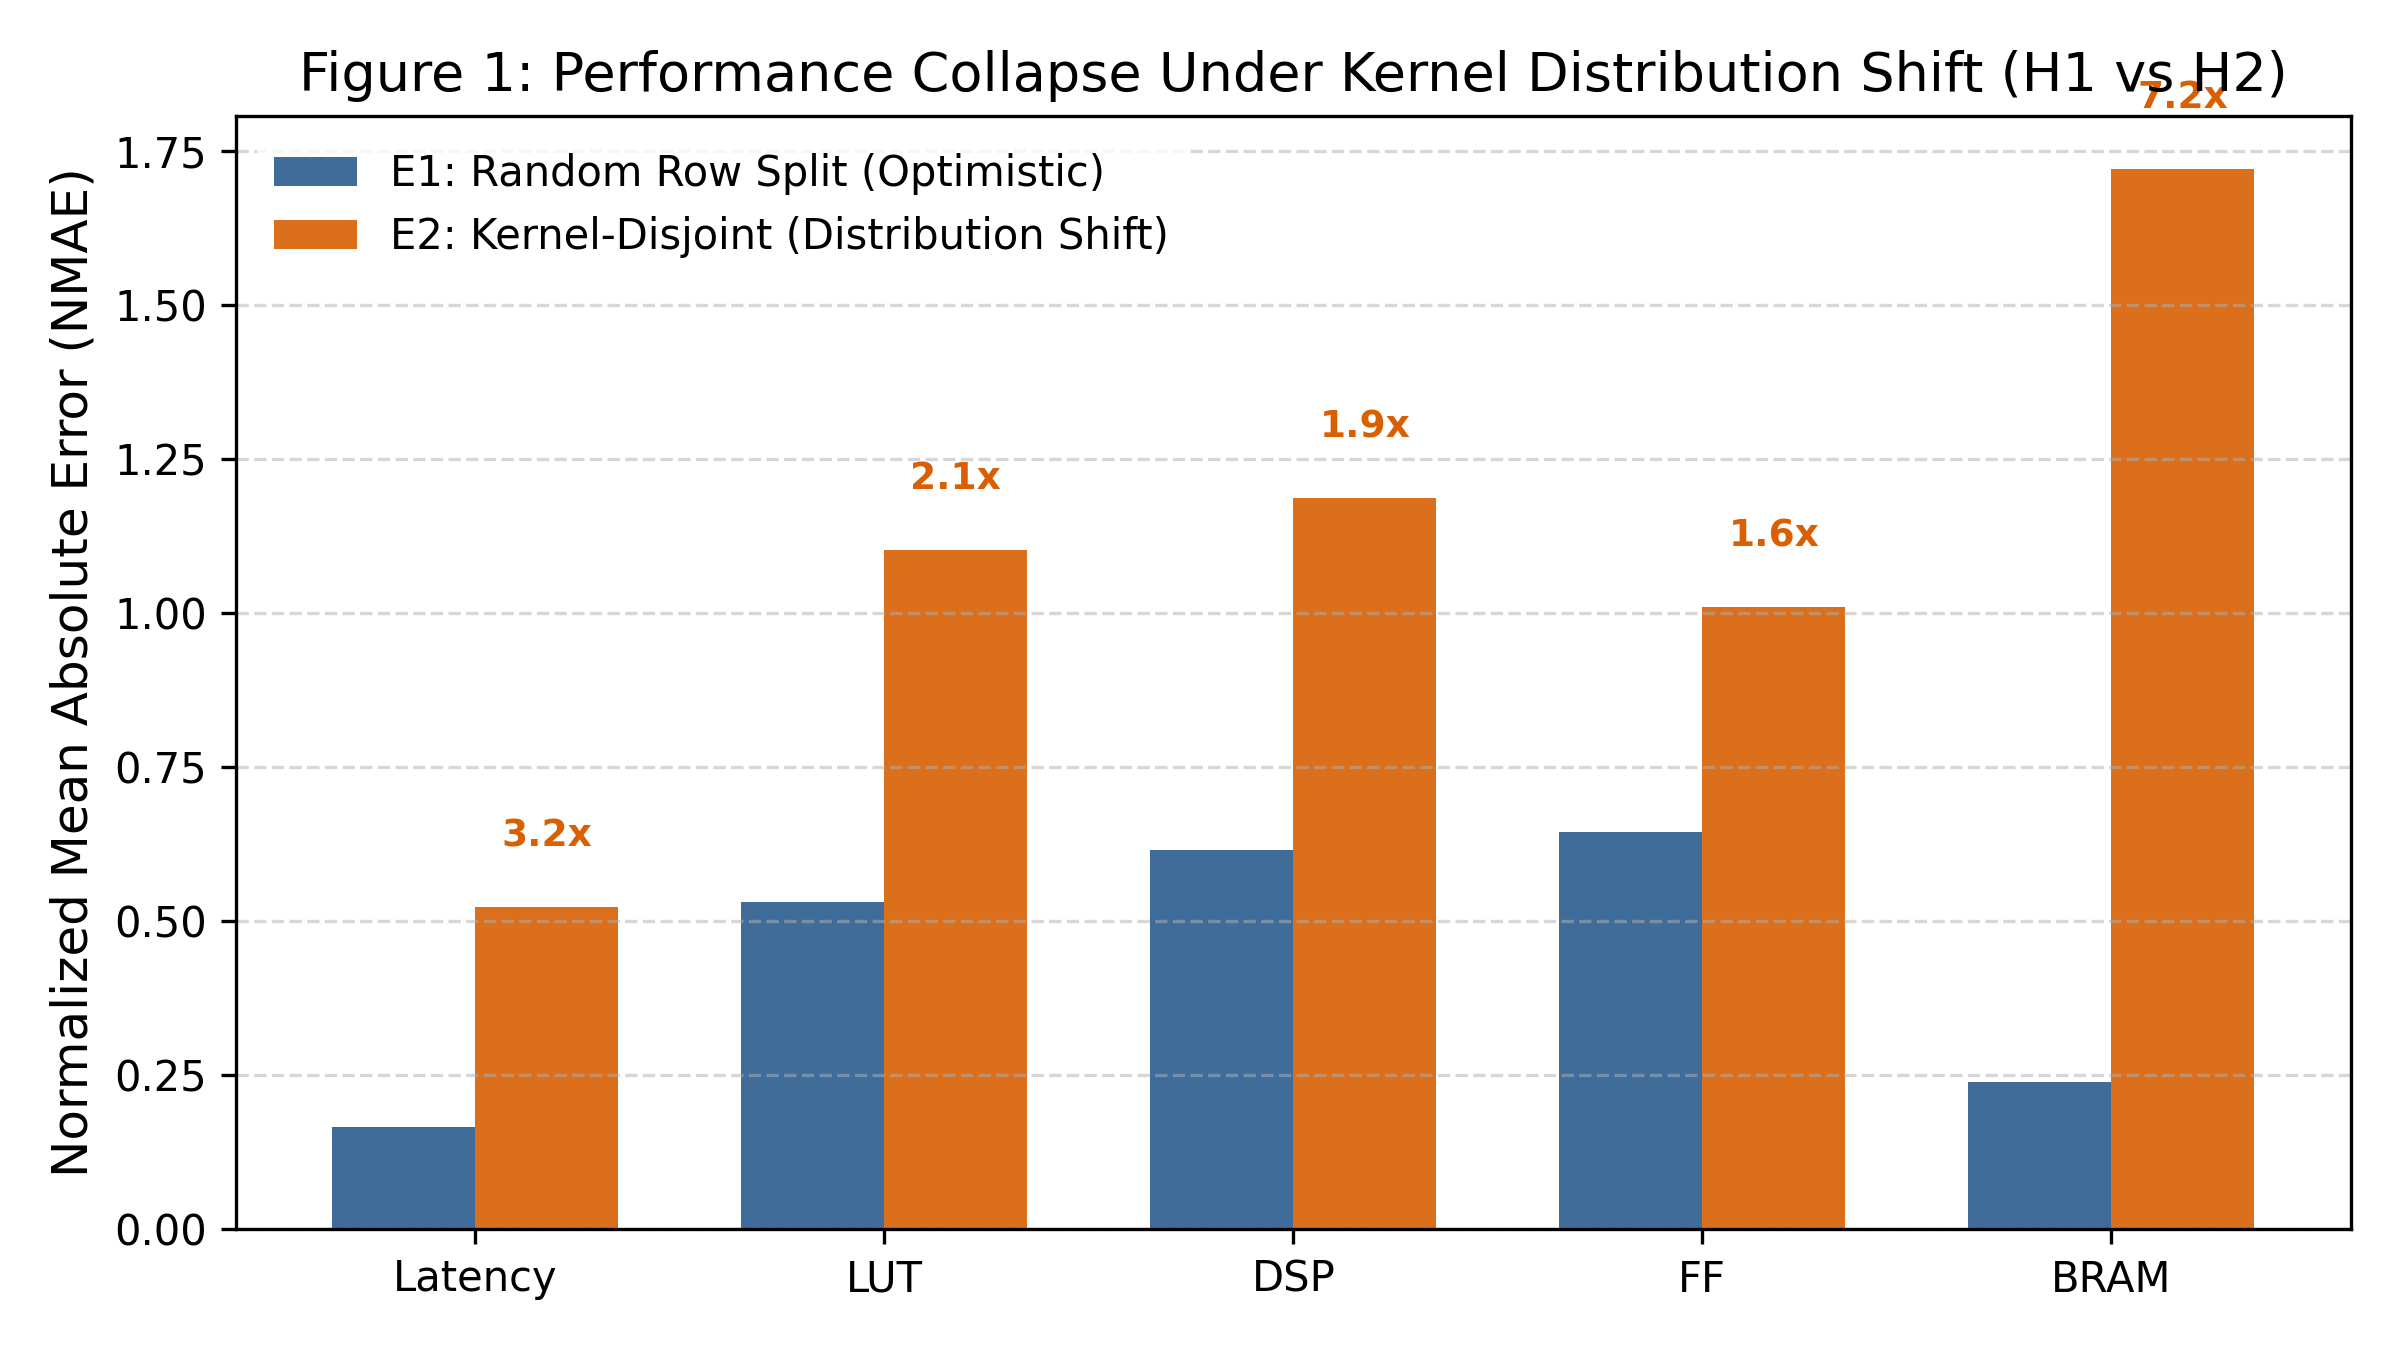
\includegraphics[width=\columnwidth]{fig1_distribution_shift_e1_vs_e2.png}
\caption{Random-row versus kernel-disjoint normalized MAE; annotations show the E2/E1 NMAE ratio.}
\label{fig:shift}
\end{figure}

\begin{figure}[t]
\centering
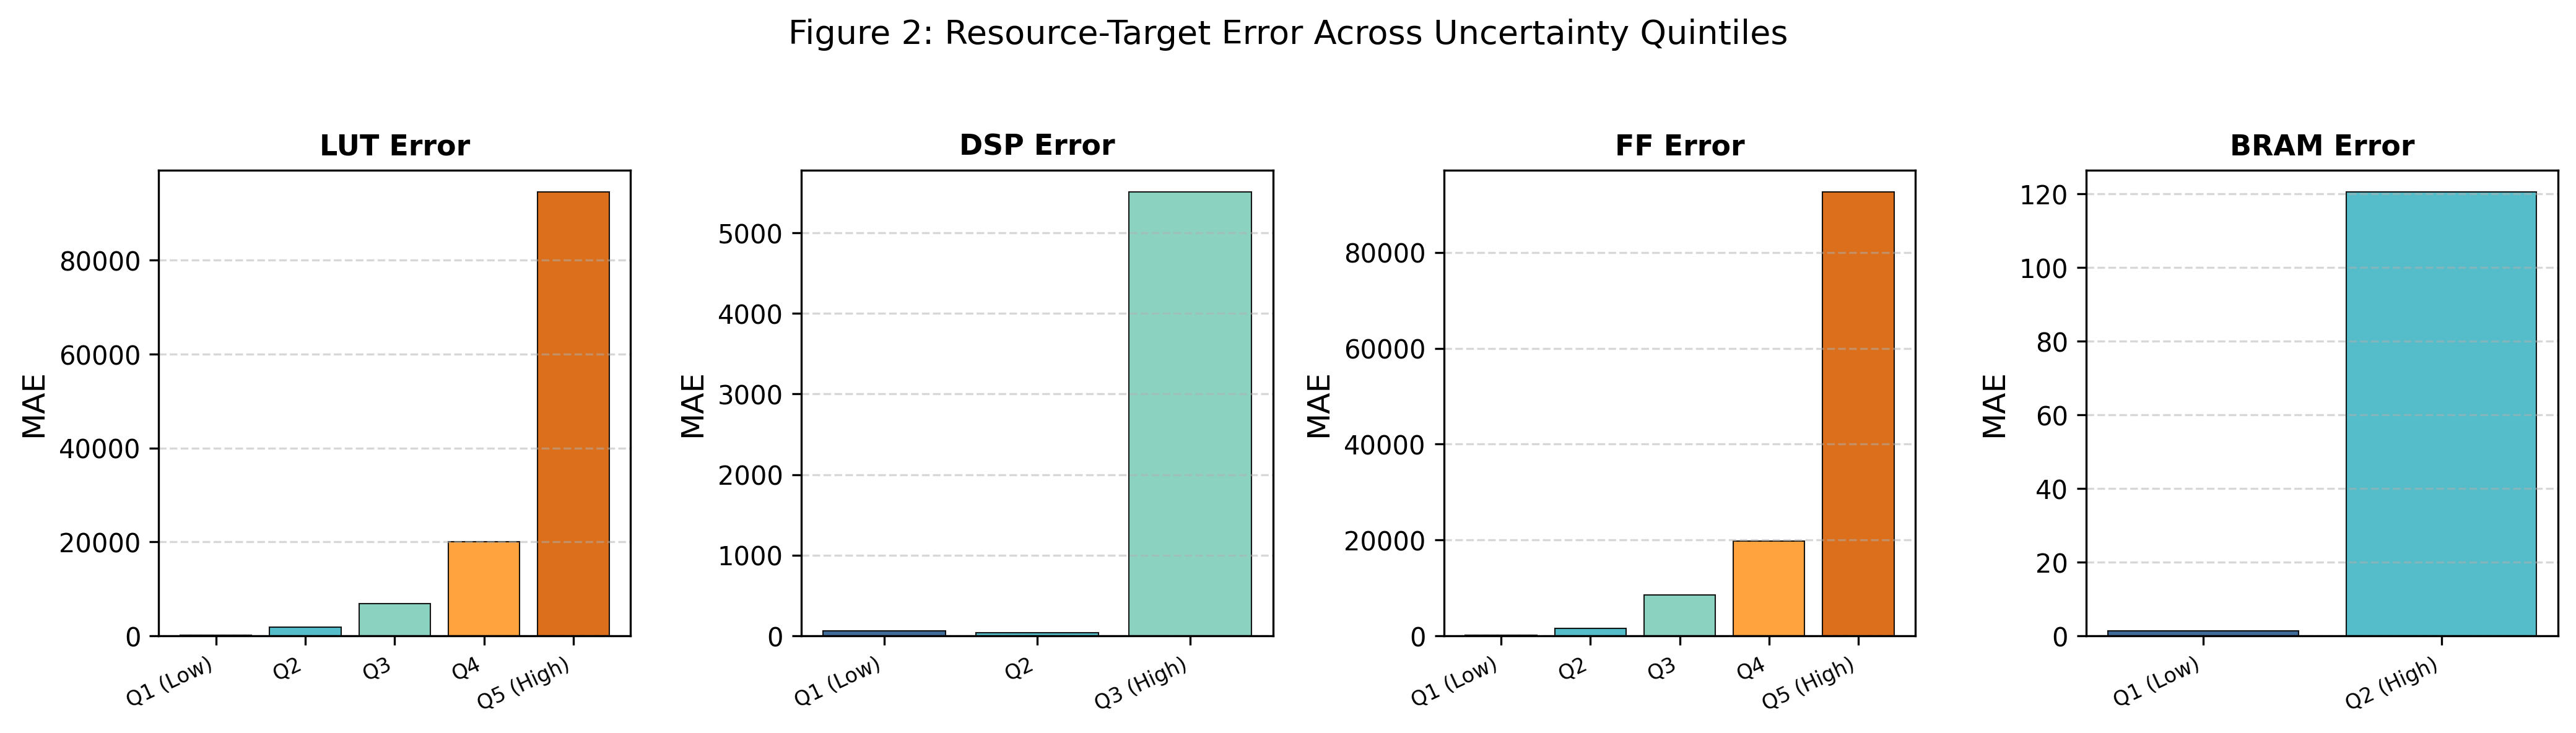
\includegraphics[width=\columnwidth]{fig2_uncertainty_correlation_quintiles.png}
\caption{Mean absolute error across tree-uncertainty quintiles for LUT, DSP, FF, and BRAM; latency is reported in Table~\ref{tab:uq}.}
\label{fig:uq}
\end{figure}

\begin{figure}[t]
\centering
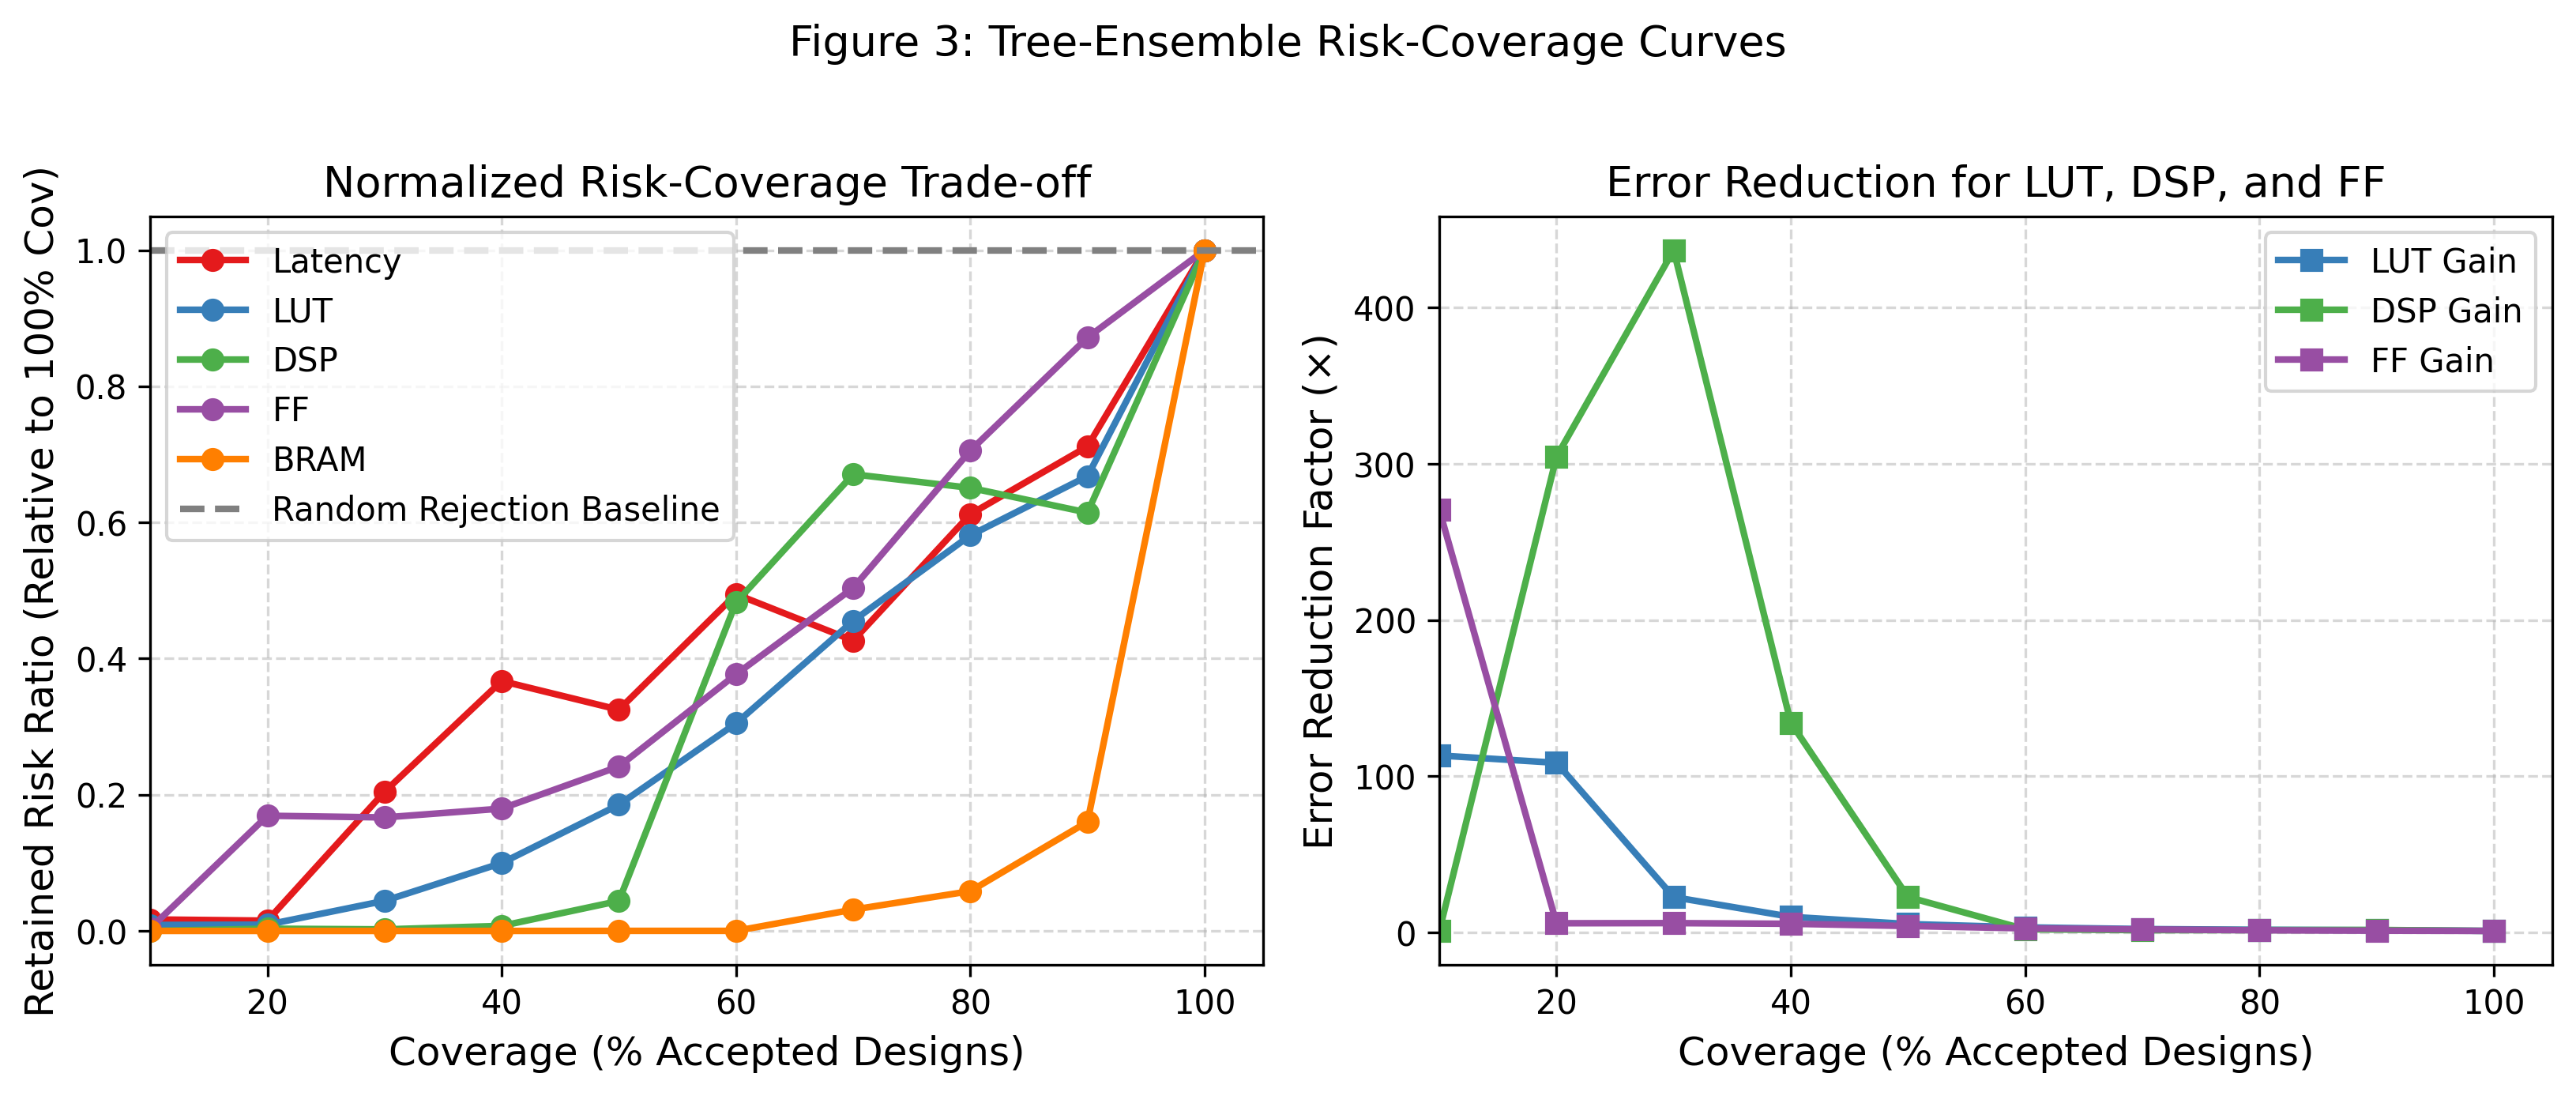
\includegraphics[width=\columnwidth]{fig3_risk_coverage_curves.png}
\caption{Tree-ensemble risk--coverage curves. BRAM error-reduction factors are omitted because zero-valued retained errors make ratios unstable.}
\label{fig:risk}
\end{figure}

\subsection{Feature ablation}
The feature ablation reveals a distinction between point accuracy and uncertainty ranking. Set C, which combines structural and pragma features, gives the strongest uncertainty--error Spearman correlation for each target in the saved ablation table, but its grouped point-prediction $R^2$ is poor for several resource targets, including LUT ($-11.643$), DSP ($-15.064$), and FF ($-2.004$). Figure~\ref{fig:ablation} therefore must not be interpreted as evidence that Set C is the best QoR predictor. It shows that features useful for ranking uncertainty need not be the same features that minimize point-prediction error.

\begin{figure}[t]
\centering
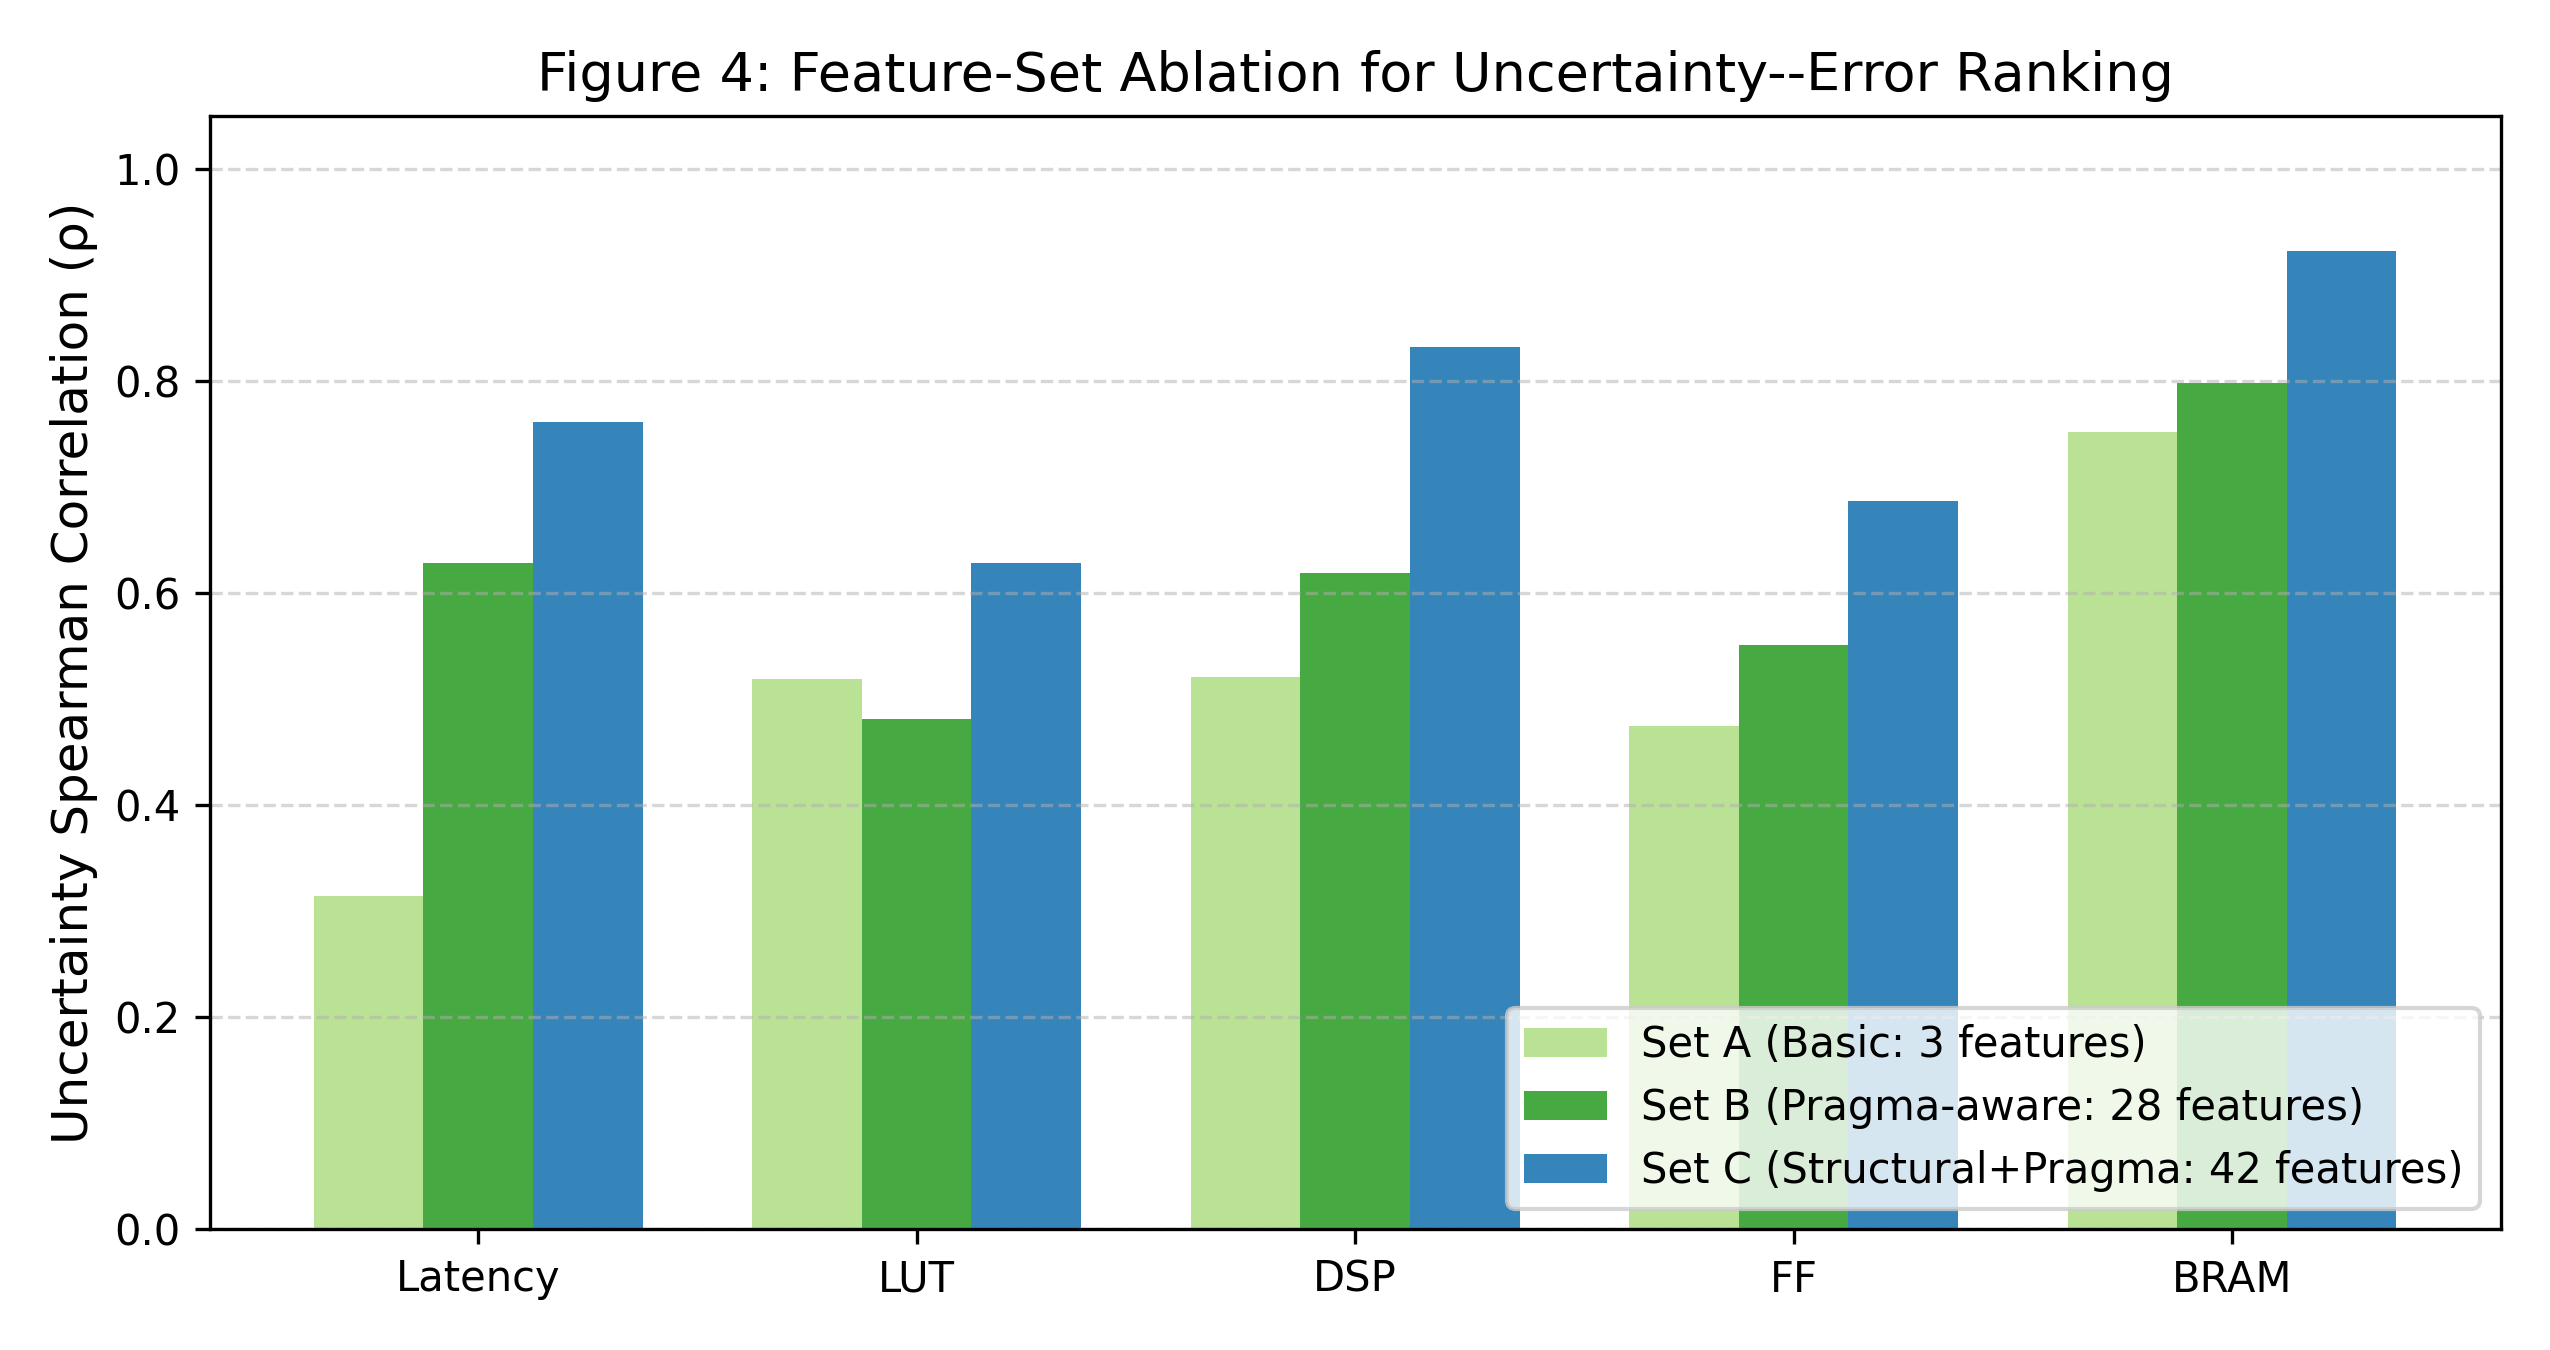
\includegraphics[width=\columnwidth]{fig4_feature_ablation.png}
\caption{Feature-set ablation for uncertainty--error ranking; this figure does not show point-prediction accuracy.}
\label{fig:ablation}
\end{figure}

\subsection{Validation-only tuning}
Compact validation-only tuning does not produce a universal improvement. Across E3, tuned Gradient Boosting improves latency $R^2$ modestly to $0.386\pm0.240$, but its latency LogMAE is $1.645\pm0.226$, worse than the fixed baseline. Improvements are target-dependent: FF and BRAM LogMAE improve slightly, while other targets do not consistently improve. The two-stage zero-aware DSP model obtains positive-class F1 near 0.847 in E2, but does not dominate the regression metrics. Accordingly, tuning is treated as a supporting analysis rather than the paper's main contribution.

\section{Discussion}
The experiments reveal three practical lessons. First, row-level random splits can conceal the real generalization problem because related configurations of one kernel occur in both partitions. Second, latency is more predictable than the resource targets under the present feature representation and group shift; negative or near-zero resource $R^2$ values are meaningful evidence rather than failures to hide. Third, uncertainty can be operationally useful even when point accuracy is limited: high uncertainty identifies predictions with larger expected error. Calibration nevertheless requires separate attention, especially for heavy-tailed latency and zero-heavy BRAM/DSP.

This work should therefore be positioned as a reliability and evaluation framework, not as a claim of state-of-the-art point accuracy. The results do not establish universal superiority of tuned models, perfect calibration, or deployment safety in a security-critical system.

\section{Threats to Validity and Limitations}
\begin{itemize}
    \item The study uses one public ForgeHLS release and one grouping rule. Other datasets and semantic kernel identities may produce different shift behavior.
    \item The source--algorithm pair is an auditable proxy for logical kernel identity, not a proof of semantic equivalence.
    \item Tree and deep-ensemble uncertainty are practical surrogates; they are not formal guarantees of calibrated predictive intervals. The observed tree association is partly confounded by predicted scale, and the deep ensemble does not consistently improve selective prediction.
    \item Resource targets are zero-heavy and latency is heavy-tailed, so raw MAE, $R^2$, and error ratios require careful interpretation.
    \item The security symposium scope shown in the call for papers is broader than HLS QoR prediction. This manuscript should only be submitted there if the organizers explicitly accept trustworthy-AI/HLS methodology; otherwise, an EDA, hardware design, or trustworthy-ML venue is a better fit.
\end{itemize}

\section{Reproducibility}
The complete workflow regenerates the feature matrix and split files from the original JSON data, checks required fields, asserts zero group overlap for E2/E3, trains baselines before uncertainty analysis, and exports CSV, NPZ, figure, and table artifacts. The repository contains the scripts and the Colab notebook used for the verified run. Before submission, the authors should archive the exact dataset release identifier, Python/package versions, notebook, commit hash, and final output checksums.

\section{Conclusion}
We presented a leakage-controlled reliability study of multi-objective HLS QoR prediction under kernel-level distribution shift. On 184,717 real ForgeHLS records, random row splits substantially overestimate resource-target generalization relative to kernel-disjoint evaluation. Repeated grouped evaluation shows that latency is the strongest target, while resource prediction is weak and unstable. Tree disagreement provides strong error ranking across all targets, and selective prediction can prioritize lower-risk designs, but calibration remains target-dependent. These findings support a reliability-first methodology for HLS surrogate modeling and caution against reporting random-split accuracy as evidence of deployment-ready generalization.

\bibliographystyle{IEEEtran}
\bibliography{references}

\end{document}
